\subsection{Numberlink (AKA Flow Free) puzzle as a MaxSAT problem + toy \ac{PCB} router}

% TODO \ref{}
Let's revisit my solution for Numberlink (AKA Flow Free) puzzle written for Z3Py.

What if holes in the puzzle exist?
Can we make all paths as short as possible?

I've rewritten the puzzle solver using my own SAT library 
and now I use \href{http://sat.inesc-id.pt/open-wbo/}{Open-WBO MaxSAT solver},
see the source code, which is almost the same: \url{https://github.com/DennisYurichev/SAT_SMT_by_example/blob/master/puzzles/numberlink/MaxSAT/numberlink_WBO.py}.

But now we ``maximize'' number of empty cells:

% TODO join these figures side-by-side:

\begin{figure}[H]
\centering
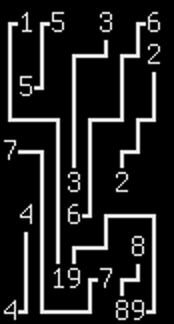
\includegraphics[scale=0.5]{puzzles/numberlink/MaxSAT/MaxSAT.png}
\caption{}
\end{figure}

This is a solution with shortest possible paths. Others are possible, but their sum wouldn't be shorter.
This is like toy \ac{PCB} routing.

What if we comment the \TT{s.fix\_soft\_always\_true(cell\_is\_empty[r][c], 1)} line and set \TT{maxsat=True}?

\begin{figure}[H]
\centering
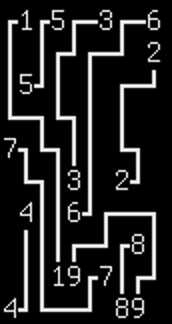
\includegraphics[scale=0.5]{puzzles/numberlink/MaxSAT/SAT.png}
\caption{}
\end{figure}

Lines 2 and 3 ``roaming'' chaotically, but the solution is correct, under given constraints.

The files: \url{https://github.com/DennisYurichev/SAT_SMT_by_example/tree/master/puzzles/numberlink/MaxSAT}.

